\section{Overview}\label{overview}

The CEBAF Large Acceptance Spectrometer for operation at 12 GeV beam energy (CLAS12) \cite{clas12-nim} in Hall B at
the Thomas Jefferson National Accelerator Facility (Jefferson Lab) was designed to study
electro-induced nuclear and hadronic reactions by providing efficient detection of charged and neutral particles over a large
fraction of the full solid angle.
CLAS12 is based on two superconducting magnets and multiple detector subsystems that provides large
coverage for the detection of charged and neutral particles produced by the interaction of the electron beam
from the JLab CEBAF accelerator with a target located at the center of the spectrometer. A six-coil torus
magnet defines the six-sector structure of the so-called Forward Detector that is outfitted with Drift
Chambers~\cite{dc-nim} for charged particle tracking and multiple detector systems for particle identification.
These detectors include threshold Cherenkov Counters~\cite{ltcc-nim, htcc-nim} and Ring-Imaging Cherenkov
Counters~\cite{rich-nim}, scintillator-based time-of-flight hodoscopes~\cite{ftof-nim}, and electromagnetic
calorimeters~\cite{ec-nim}. In the target region, a 5~T superconducting solenoid surrounds a central tracker
based on silicon and Micromegas detectors \cite{svt-nim,mm-nim}, and subsystems for particle identification
that include a time-of-flight scintillation counter barrel~\cite{ctof-nim} and a neutron detector~\cite{cnd-nim},
forming the so-called Central Detector.

A model representation of the CLAS12 spectrometer identifying the Forward
and Central Detectors is shown in ~\F{clas12-model}. In between the central and forward region, the CLAS12 Forward Tagger~\cite{ft-nim}
extends the kinematic coverage for the detection of electrons and photons at polar angles from 2$^\circ$ to
5$^\circ$. The total number of
readout channels of CLAS12 is larger than 100k. Typical trigger rates are 15 kHz. In 2018, data rates of
500~MB/s with a live time of $>$ 95\% were achieved.

\begin{figure}
	\centering
	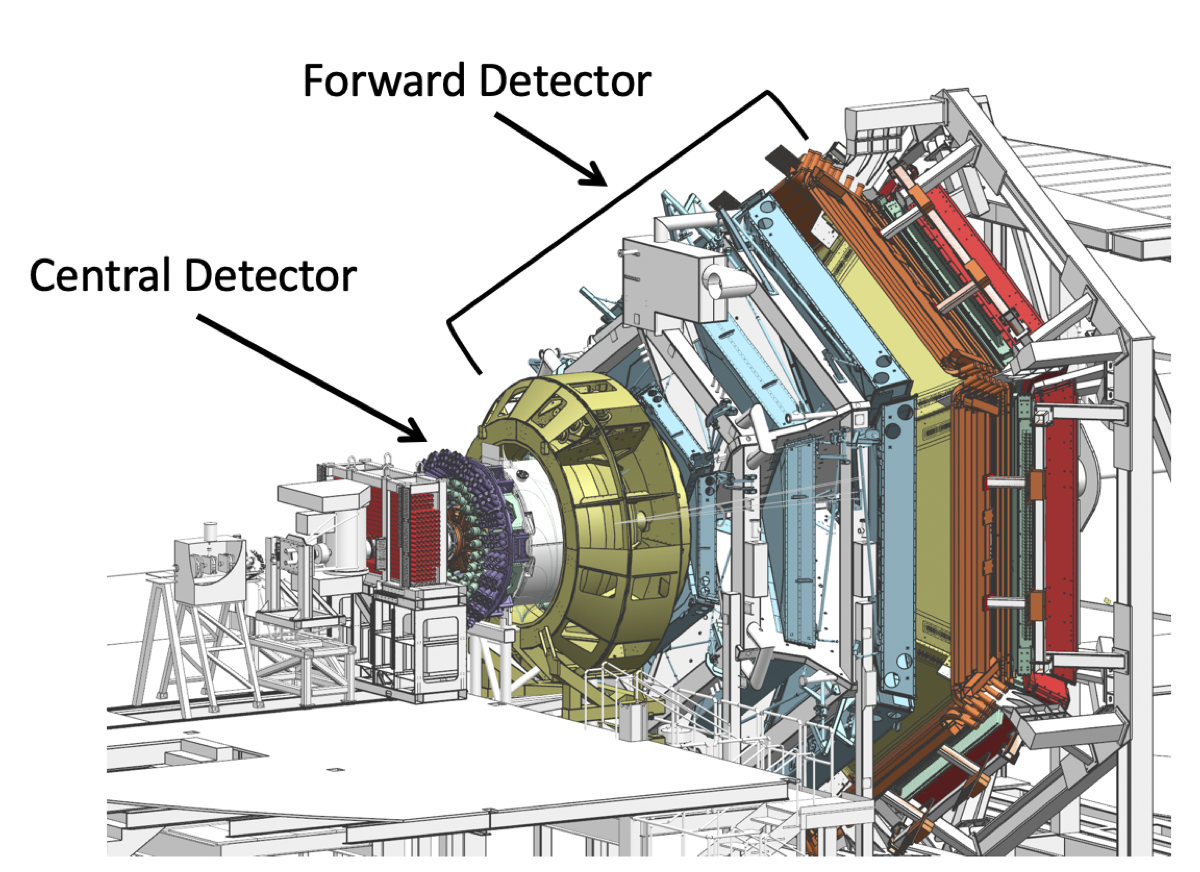
\includegraphics[width=1.0\columnwidth,keepaspectratio]{img/clas12-model.png}
	\caption{ Model representation of the CLAS12 spectrometer in Hall~B at Jefferson Laboratory. The electron
              beam is incident from the left side of this figure. The CLAS12 detector is roughly 20~m in scale along the
              beam axis. The CLAS12 Forward and Central Detectors are identified.}
        \label{fig:clas12-model}
\end{figure}

The spectrometer has met the performance criteria of instantaneous luminosity up
to \cLuminosity and momentum resolution $\sigma_p/p$ in the forward direction using the drift chambers and in the central
direction using the vertex tracker of $< 1\%$ and $< 3\%$, respectively.

The CLAS Collaboration has implemented a detector simulation within the GEMC software framework \cite{GEMC}.
During the design phase of the various CLAS12 detectors, shielding, magnets, and passive elements, GEMC allowed for studies of the
performance of the various components with respect to the desired science objectives.
GEMC enabled the optimization of the design from trade-off studies between variation of the hardware setup and placement,
and various materials and shielding thicknesses.
In addition, it was instrumental in determining the rates, PMT currents, and radiation doses to ensure that the various detectors
would survive operations during the expected spectrometer lifetime.
Before and during the experiment data taking, GEMC was instrumental in preparing and understanding the calibration
and measurements of the CLAS12 detectors.
Finally, GEMC is used to accurately calculate the CLAS12 acceptance, including the detector response, geometrical acceptance,
and tracking efficiency needed for the physics results and science goals.


GEMC is a C$^{++}$ framework that uses Geant4 \cite{geant4} to simulate the passage of particles through matter. It provides:
\begin{itemize}
	\item an application-independent geometry description;
	\item an easy interface to build/run experiments;
	\item CAD/GDML imports.
\end{itemize}

The simulation parameters are stored in external databases and are used to define the Geant4 objects at run time. This includes:
\begin{itemize}
	\item geometry;
	\item materials;
	\item mirrors;
	\item physics list;
	\item database constants;
	\item digitization to match the data numerical format;
	\item electromagnetic fields.
\end{itemize}

Particles are transported through the detector materials and produce radiation, hits, and secondaries.
GEMC then collects the Geant4 results and produces the output specified by the user.
The design of the framework is summarized in \F{gemcDesign}.

\begin{figure}
	\centering
	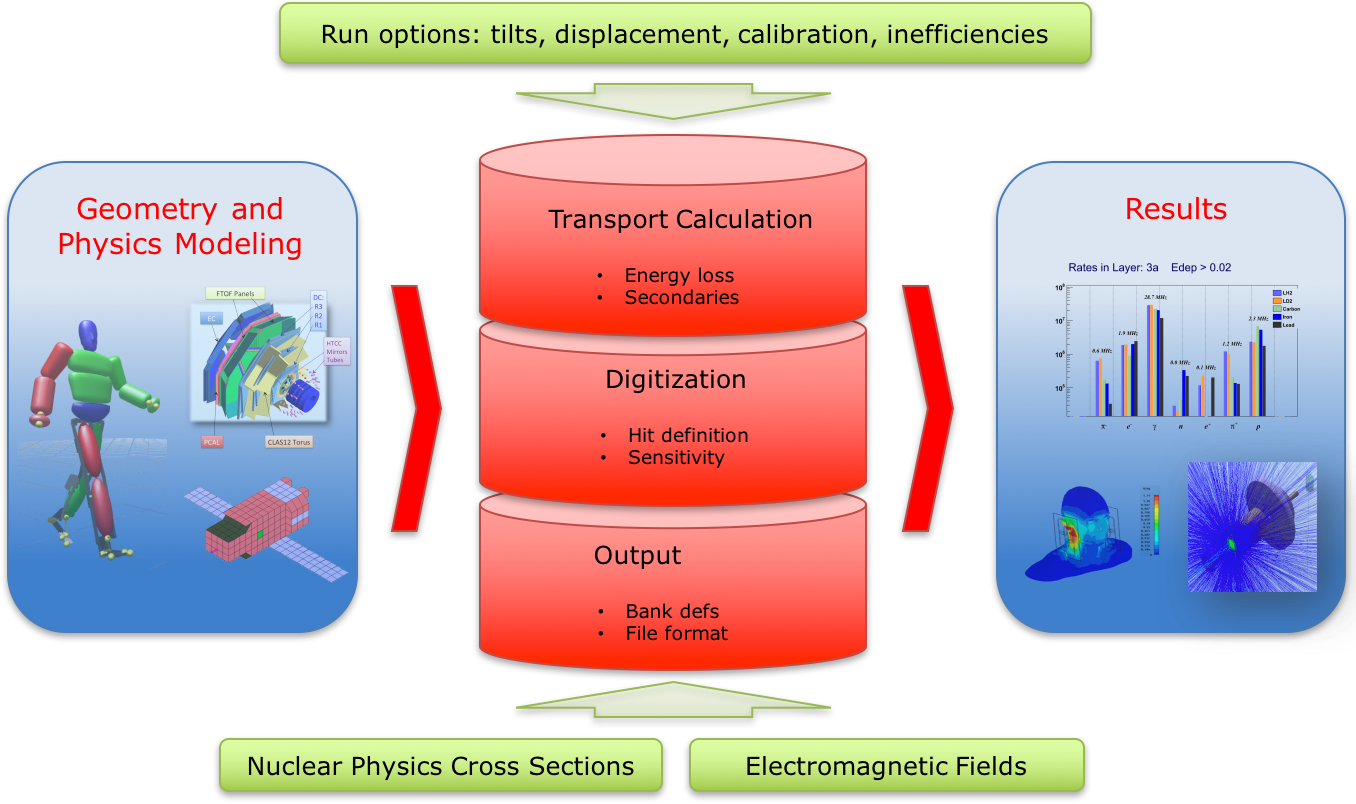
\includegraphics[width=1.0\columnwidth,keepaspectratio]{img/gemcDesign.png}
	\caption{The architecture of GEMC. The simulation parameters are stored in an external database. GEMC collects
             them and organizes the necessary Geant4 ingredients used to simulate the
             passage of particles through materials and sensitive regions. The hits are digitized with
             plugins defined by the user and collected in user-defined outputs.  }
	\label{fig:gemcDesign}
\end{figure}

The following CLAS12 systems are implemented in the simulations:

\begin{itemize}
\item Various CLAS12 targets, including liquid-hydrogen, liquid-deuterium, and various solid targets;
\item Silicon Vertex Tracker (SVT) \cite{svt-nim};
\item MicroMegas Tracker (MM) \cite{mm-nim};
\item Central Time-of-Flight System (CTOF) \cite{ctof-nim};
\item Central Neutron Detector (CND) \cite{cnd-nim};
\item High Threshold Cherenkov Counter (HTCC) \cite{htcc-nim};
\item Forward Tagger (FT) \cite{ft-nim};
\item Drift Chamber System (DC) \cite{dc-nim};
\item Low Threshold Cherenkov Counter (LTCC) \cite{ltcc-nim};
\item Forward Time-of-Flight System (FTOF) \cite{ftof-nim};
\item ElectroMagnetic Shower Calorimeter (EC) \cite{Amarian:2001zs};
\item Pre-Shower Calorimeter (PCAL) \cite{ec-nim};
\item Ring Imaging Cherenkov Detector (RICH) \cite{rich-nim};
\item Beamline \cite{beamline-nim};
\item Superconducting Magnets \cite{magnets-nim}.
\end{itemize}

The CLAS12 mechanical design include electronics, support structures, and additional hardware that cannot
entirely be imported in the simulation due memory and cpu limitations: each object increases the overall
system complexity, the time, and the memory needed to process events. Nevertheless, all the elements in
the way of particle trjectory paths to any of the CLAS12 detectors are included in the simulation.
In addition, the simulation incorporates selected hardware in order to reproduce beam related
rates in the detectors to a good level of accuracy, with priority given to volumes near high background
areas and near sensitive detectors.

By omitting some materials, we limit the ability of the simulation to make predictions. However, built in the
simulation is the ability to merge hits using random trigger events from experimental data, which include the
real background rates, as detailed in \ref{bmerging}.

The simulation implementation is detailed in the sections below.

\subsection{Geometry and Materials Import}

The geometry and system materials are stored in external databases that can be MYSQL tables or text files that
mimic the MYSQL tables. The databases can be defined using the following factories:

\begin{itemize}
	\item GEMC native API (Perl or Python);
	\item JAVA algorithms used by both simulation and the CLAS12 event reconstruction software \cite{recon-nim} or ``JAVA geometry services'';
	\item CAD (STL, PLY formats);
	\item GDML, C$^{++}$ plugins (not used in CLAS12).
\end{itemize}



The GEMC native API and the CLAS12 geometry code source repositories are listed on the CLAS12
tags portal \cite{clas12Tags}.


\subsubsection{Importing CAD volumes from the engineering model}

The Hall B detectors and their supports are designed with 3D CAD software. This includes a reference system and the
hierarchy of all detector elements, down to details such as nuts and bolts.
The CAD models are exported into STEP files \cite{stepFiles}.
In order to import them into the GEMC simulation, the elements in the STEP file are ``tessellated'',
a process in which polygonal triangular faucets are created to define a Geant4 volume that best represents
the original CAD element.
The software used to do this is FreeCad \cite{freeCad}. An example of tessellation showing the polygonal shapes
is shown in \F{targetScatteringChamber}. The number of faucets depends on the object complexity, and varies between
100 and 10,000.
Not all the objects are imported from the enginerring model due to the following limitations:

\begin{enumerate}
\item
\item when volumes that contains very small and pointy features are tessellated, the faucets may be too small
      to be processed properly in geant4 and cause tracks to get stuck or produce swimming errors.
\end{enumerate}

\begin{figure}[h]
	\centering
	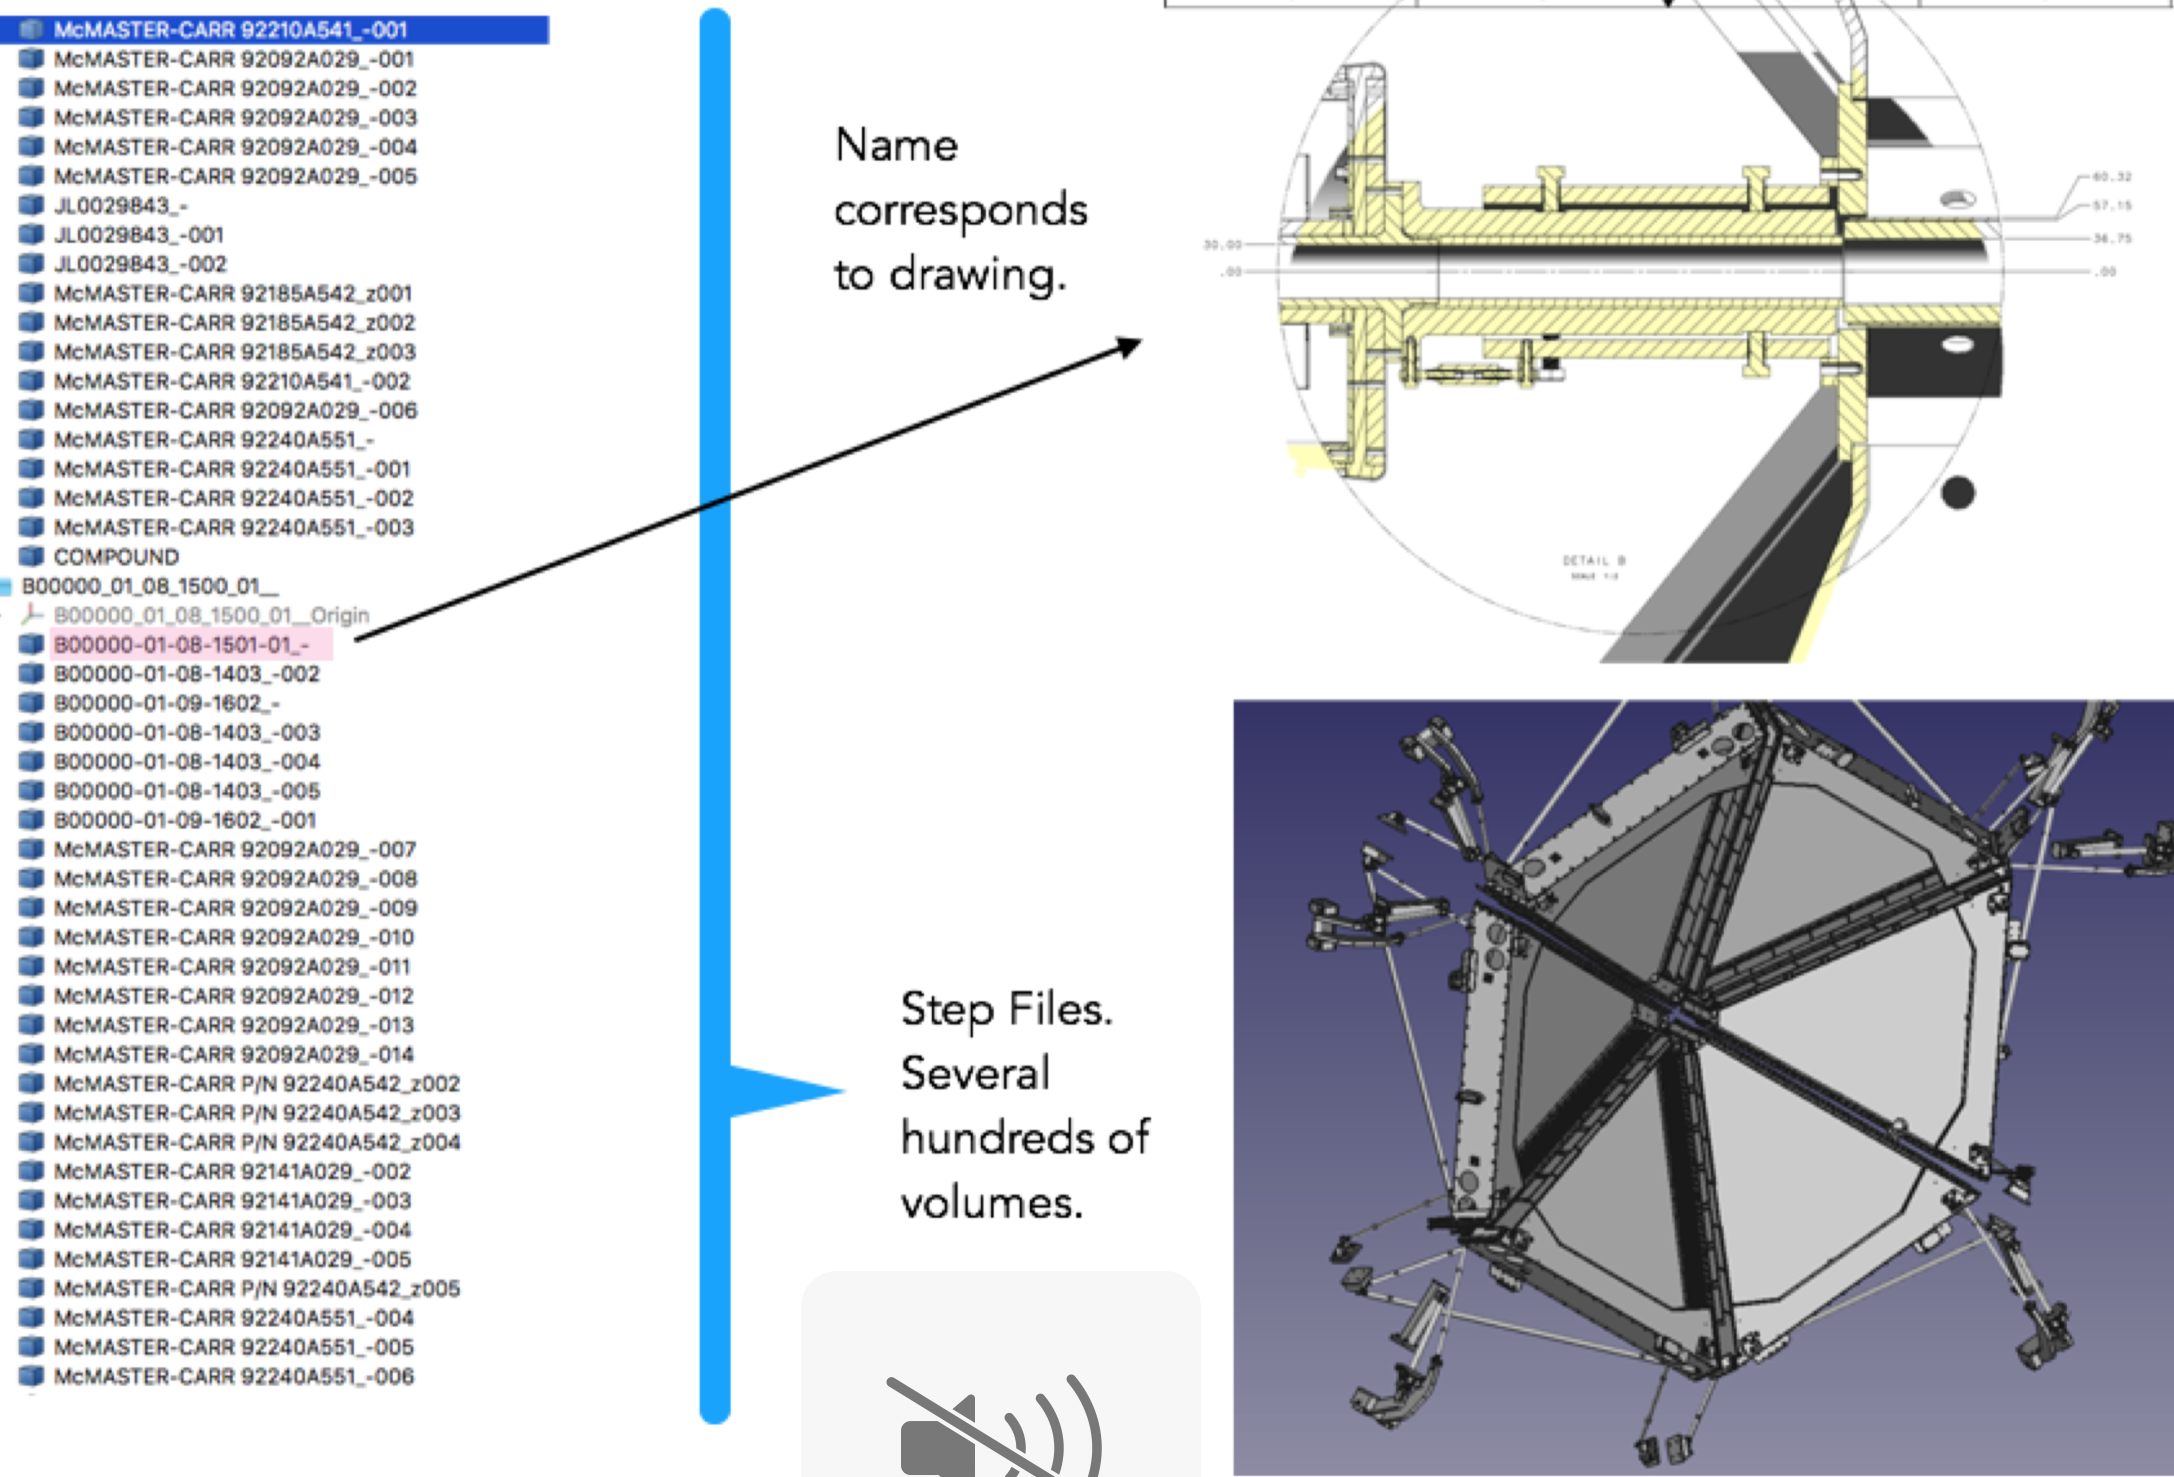
\includegraphics[width=1.0\columnwidth,keepaspectratio]{img/cadSelection.png}
	\caption{The engineering model of the CLAS12 drift chambers.
             Some hardware shown in this figure, for example the support structure outside the detector
             fiducial volume, is not imported in the simulation as explained in \ref{overview} }
	\label{fig:cadSelection}
\end{figure}

The simulated CAD import is as close to reality as the engineering model is close to reality.
We did encounter differences between the STEP files, the drawings, and reality in a few occasions and designed
a workflow to eliminate any discrepancies.
An example of the comparing volumes in the GEMC simulation to the engineering drawings
as part of the validation process is shown in \F{cadValidationExample}.

\begin{figure}
	\centering
	\includegraphics[width=0.99\columnwidth,keepaspectratio]{img/targetScatteringChamber.png}
	\caption{An example of a volume from a STEP file tessellated in GEMC. The volume that is shown is the target scattering chamber.
            Top: the CAD representation in the engineering model. Bottom: the tessellation. }
	\label{fig:targetScatteringChamber}
\end{figure}


%\begin{figure}
%	\centering
%	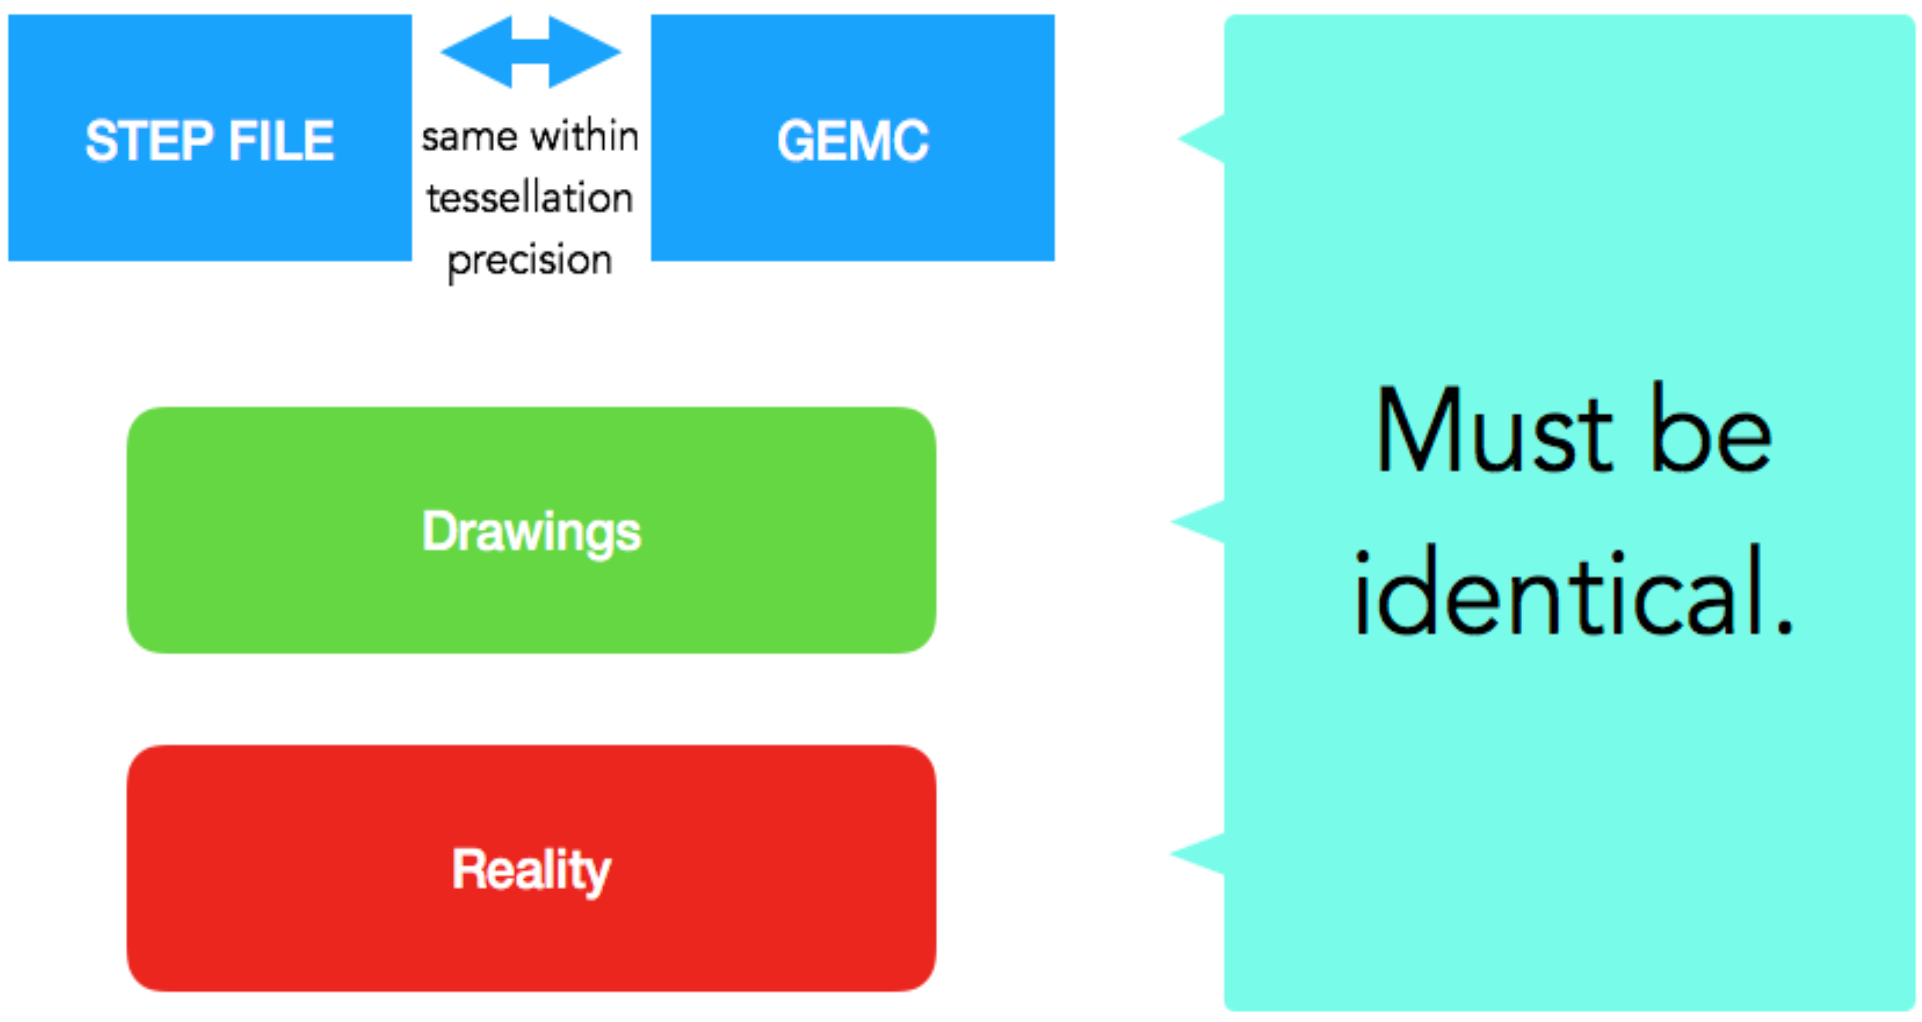
\includegraphics[width=0.99\columnwidth,keepaspectratio]{img/cadValidation.png}
%	\caption{There are four possible representation of a volume: the one coming from the STEP file
%            and the tessellated one are exactly the same object (within the tessellation precision).
%             In some cases, certain elements and their sizes and positions did not match the drawings.
%             In other cases, they did not match what was built and measured, or their position did not
%             match the survey. To eliminate these occurrences physicists and engineers worked until
%             the final iteration of a volume was the same in all 4 models: STEP/GEMC, Drawings and Reality}
%	\label{fig:cadValidation}
%\end{figure}


\begin{figure}
	\centering
	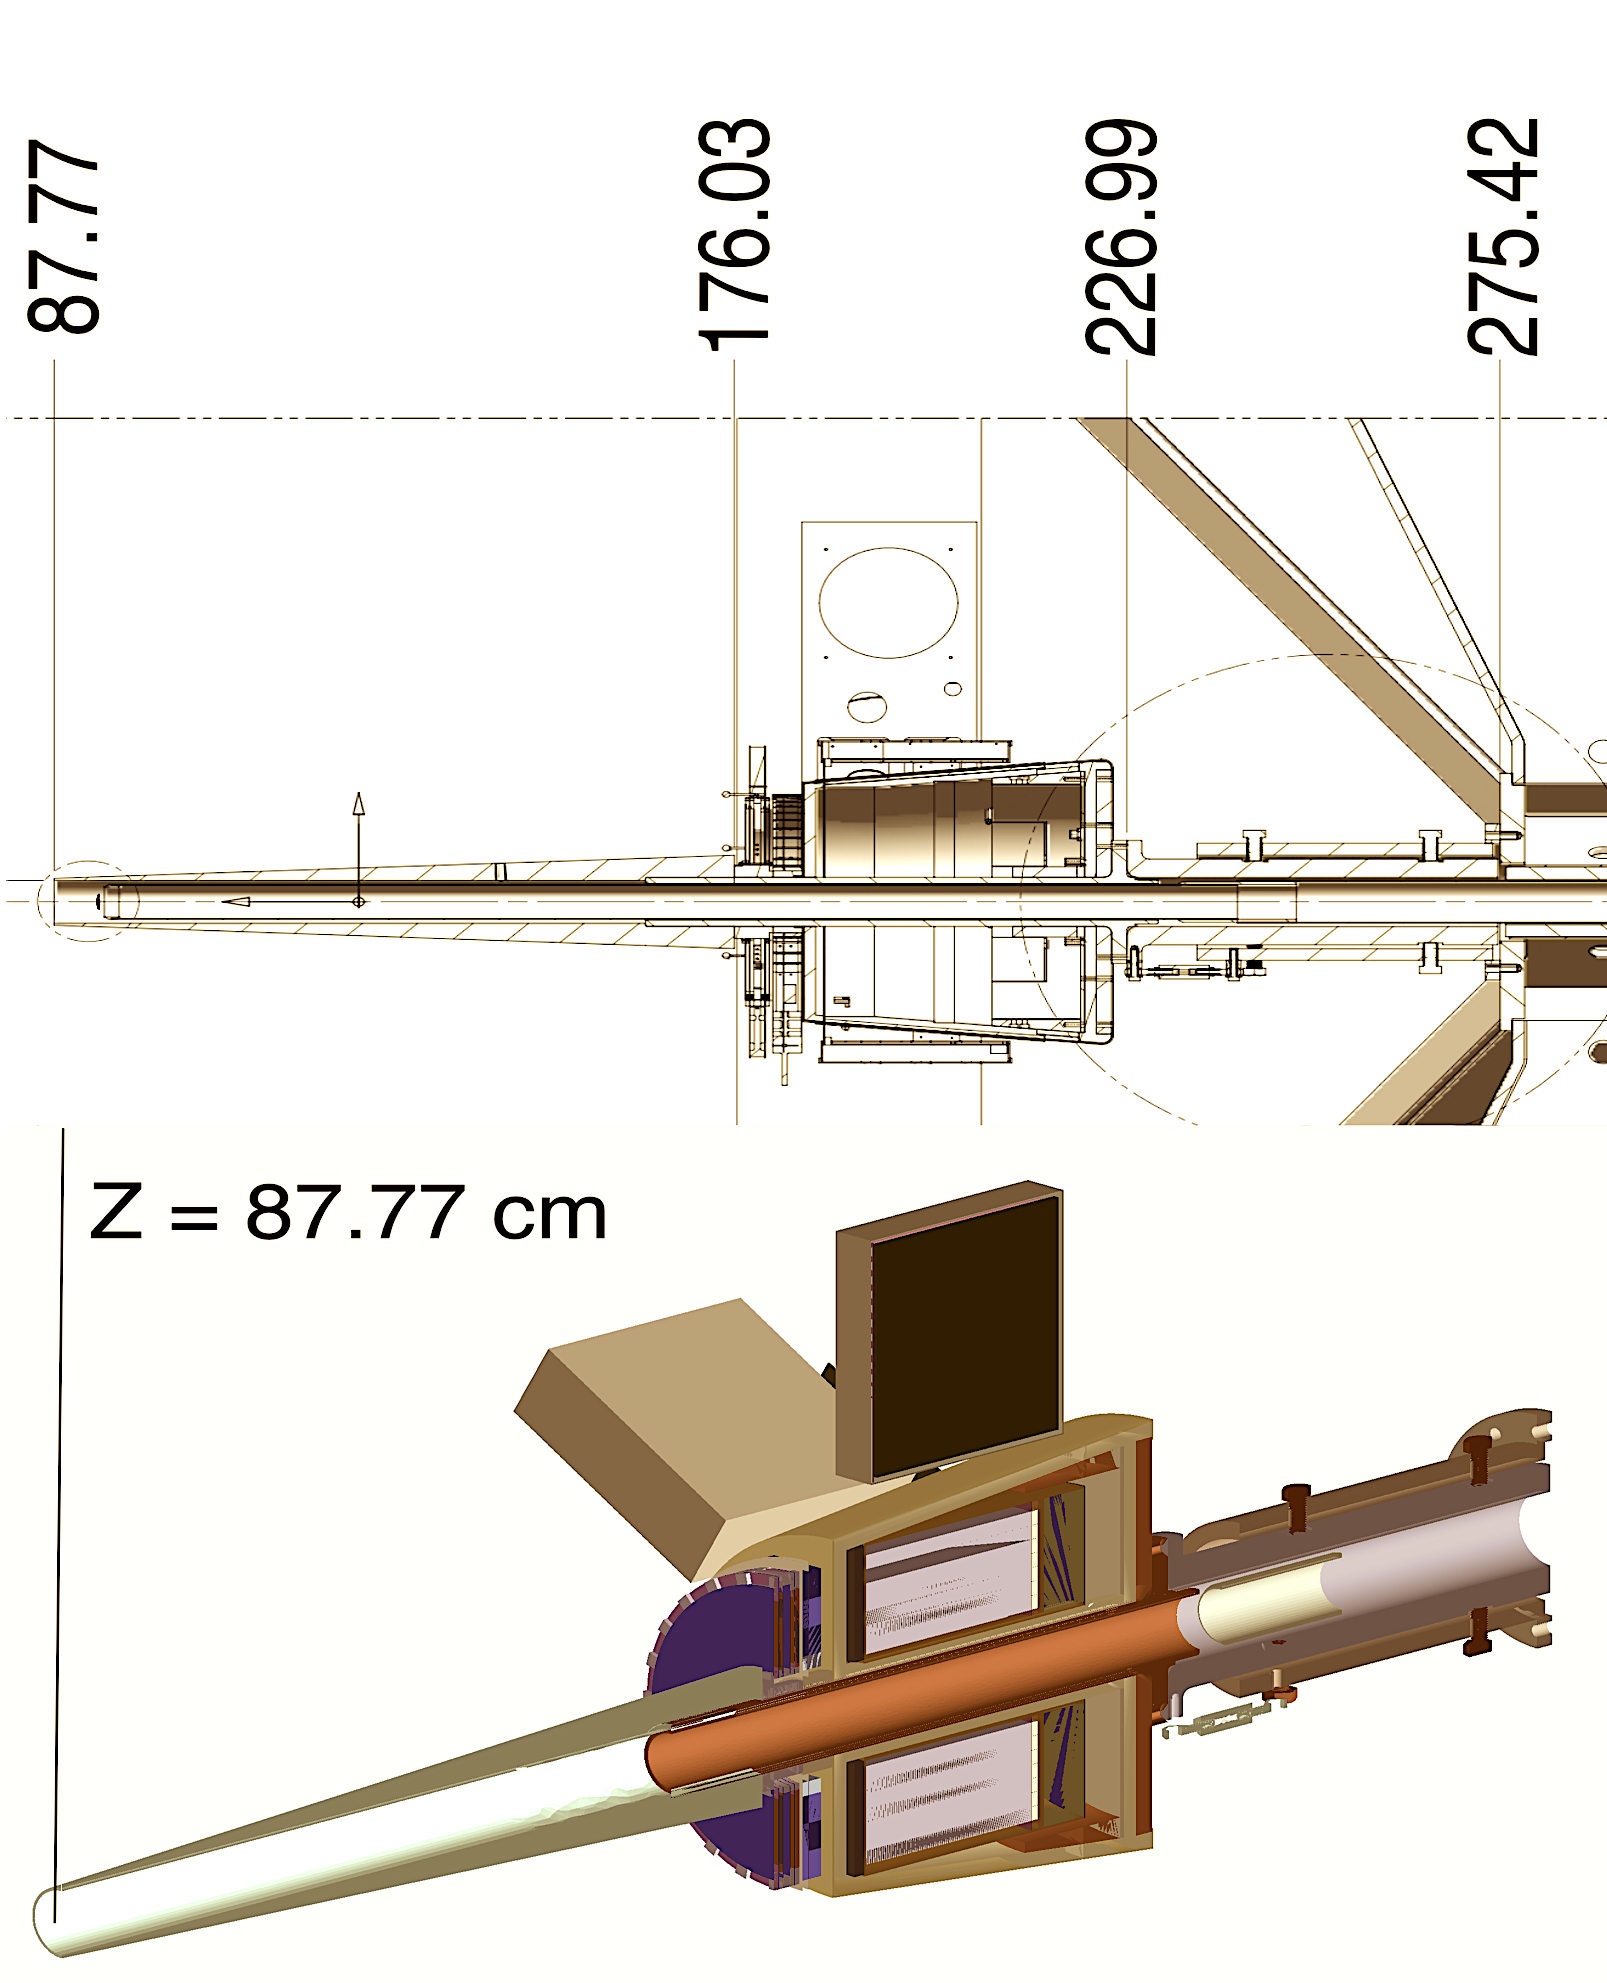
\includegraphics[width=0.99\columnwidth,keepaspectratio]{img/cadValidationExample.png}
	\caption{An example of comparing volumes in the GEMC simulation to the engineering drawings, in this case to validate the cone shield
             position. Top: engineering drawings of the CLAS12 beamline and shielding. The start of the M\o ller shielding is 87.77 cm downstream
             of the target center. Bottom: a geantino (a special Geant4 particle that does not interact with materials or fields)
             is shot vertically at $z$=87.77~cm, showing that the Geant4 cone position agrees with the drawings.}
	\label{fig:cadValidationExample}
\end{figure}



\subsection{Magnetic Fields}
The magnetic fields are loaded from ASCII files. The following Geant4 parameters are loaded from
command line options or configuration files at run time:

\begin{itemize}
	\item minStep: minimum track distance in the magnetic field (step) before re-computing its value;
	\item integralAlgorithm: compute the field value from the closest cell or using a linear (or bi-linear) interpolation;
	\item interpolationMethod: interpolation algorithm used to transport tracks in magnetic fields, typically
		  a variation (choice of order and/or precision) of Runge-Kutta \cite{rungeKutta} methods.
\end{itemize}

The implementation of the CLAS12 magnetic fields is described in Section \ref{sec:clas12FieldMaps}.

\subsection{Event Time Window and Hit Definition}

The Geant4 sensitive volumes are associated with a GEMC identifier that contains hierarchical information such as mother volumes
and volume copy number.

Each detector is associated with a time quantity to mimic the readout electronic time window. The time window and identifier
define a GEMC hit from a series of Geant4 steps: all the steps in a given identifier that are within the time window
are part of the same GEMC hit. The algorithm is illustrated in \F{hitDefinition}.

\begin{figure}
	\centering
	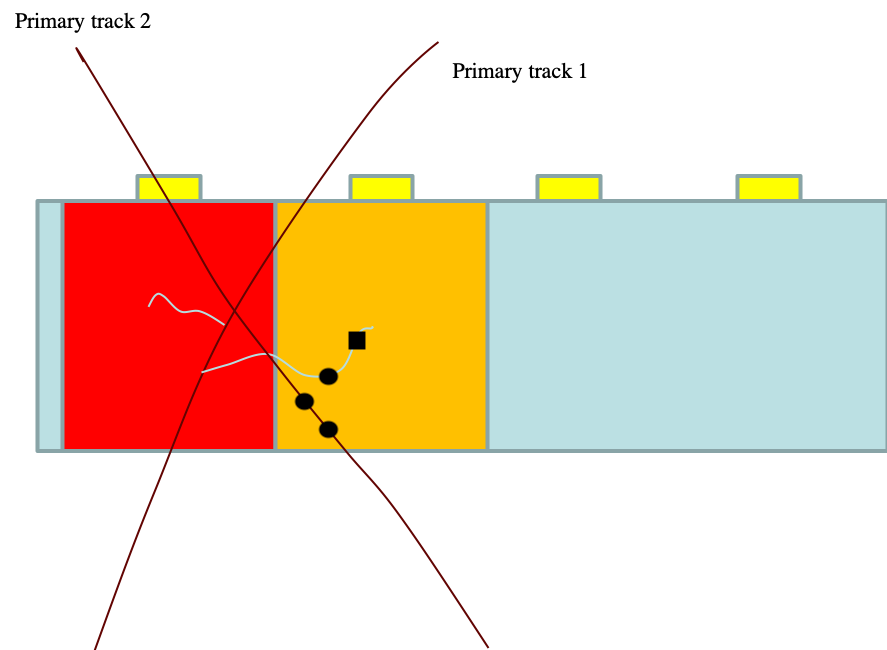
\includegraphics[width=0.99\columnwidth,keepaspectratio]{img/hitDefinition.png}
	\caption{The GEMC hit definition algorithm. The sensitive element Cell 2 is hit by three particles, two primaries and one secondary.
             The Geant4 steps are drawn explicitly with circle and triangle symbols. The circle steps generated by both the primary track 1 and the secondary
             from track 2 are within the time window and therefore are part of the same GEMC hit ``Cell 2, Hit 1''.
             The single triangle step generated by the secondary from track 2 comes after and does not fall within the ``Cell 2, Hit 1''
             time window; therefore it is part of a new GEMC hit, ``Cell 2, Hit 2''.}
	\label{fig:hitDefinition}
\end{figure}

\subsection{Process Identification}

A ``Process ID'' method can be implemented by some digitization algorithm to modify or add GEMC identifiers to each Geant4 step. For CLAS12 this happens in two
cases, detailed for each detector:

\begin{itemize}
	\item a paddle is hit but two outputs are produced because there is one PMT at each end of the scintillator. This
          is the case for CTOF, CND, and FTOF.
    \item some hardware elements are not present in the simulation. This is the case for the drift chambers, where the volumes do not contain
          the individual wires. In this case the wire number is calculated based on the position of the hit in the mother volume. In CLAS12 this mechanism
          is adopted by the DC, SVT, RICH, and MM.
\end{itemize}


\subsection{Detectors and Hit Process Plugin Mechanism}

The detectors are associated with C$^{++}$ digitization routines at run time (see \F{pluginsAssociation}).
This allows the routines to be developed independently from the core code. Abstract methods can be derived in
the individual detector hit processes to define the treatment of the Geant4 steps within the detector
time window to provide three kind of outputs:

\begin{figure}
	\centering
	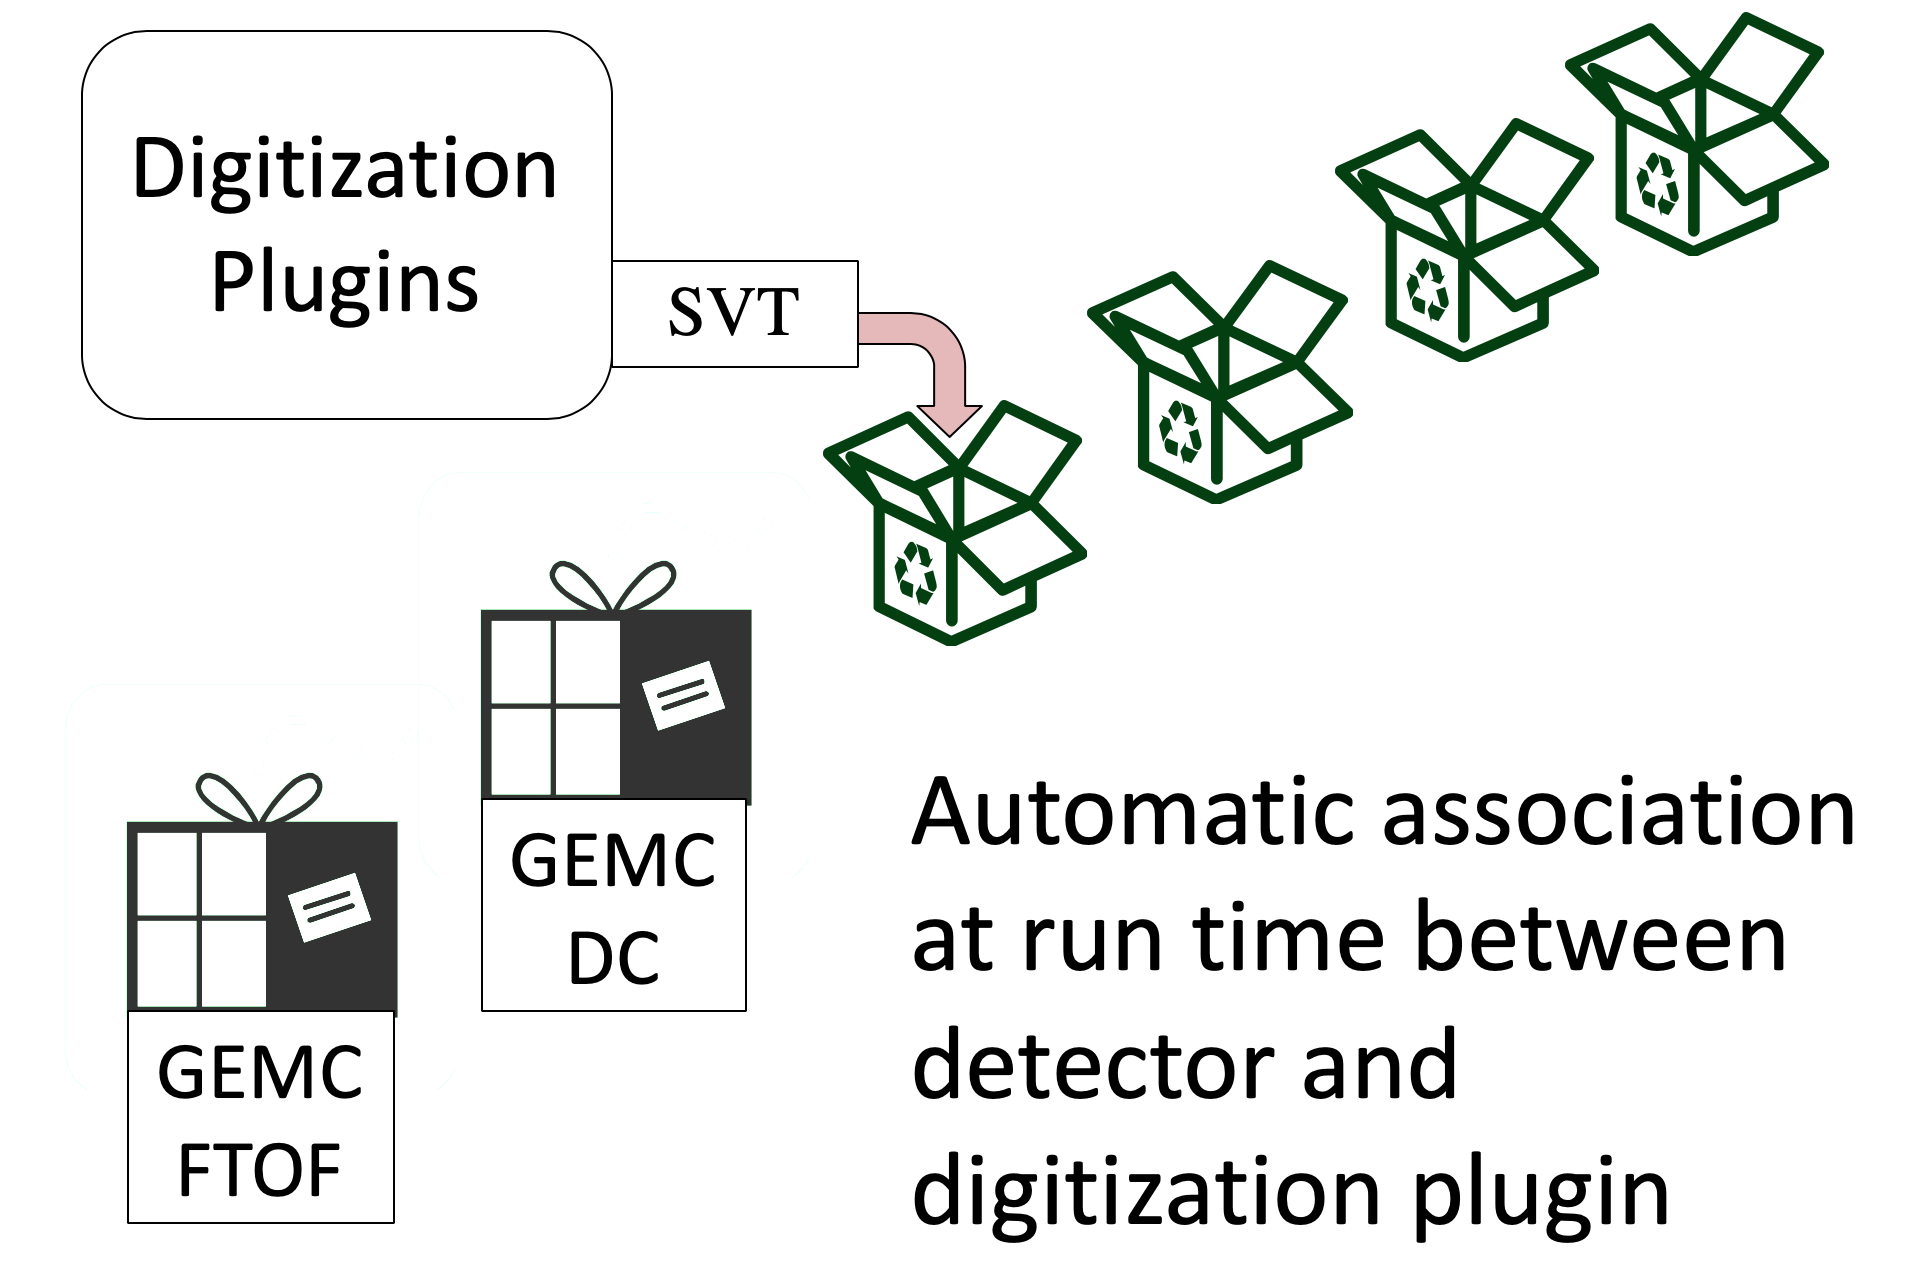
\includegraphics[width=1.0\columnwidth,keepaspectratio]{img/pluginsAssociation.png}
	\caption{Hit process digitization plugin association. The detectors are associated by name with the hit process routine
             plugins at GEMC run time. The routines are registered in the hit process map and are called during digitization.}
	\label{fig:pluginsAssociation}
\end{figure}


\begin{itemize}
	\item a bank with digitized variables for each hit;
	\item a bank with digitized variables for each Geant4 step;
	\item a bank with an analog voltage versus time signal for each Geant4 hit.
\end{itemize}

The digitized banks are detailed below for each detector subsystem.

\subsection{``True'' Information}

Various data such as particle identification, momenta, hit positions, vertex of particle, etc, (true information) is stored in memory
as the tracks progress in each detector. The true information is integrated (one variable entry per GEMC hit) and/or
verbose (one variable entry per Geant4 step). It is saved in the output at the end of each event.
The list of variables in the true information bank is summarized in Table \ref{tab:trueInformation}.

\begin{table}[h]
	\small
	\begin{center}
		\begin{tabular}{| c | c |}
			\hline \hline
			Variable    & Description  \\
			\hline
				pid         &   ID of the First Particle (FP) entering the volume \\
				mpid        &   ID of the mother of the FP \\
				tid         &   Track ID of the FP\\
				mtid        &   Track ID of the mother of the FP  \\
				otid        &   Track ID of the ancestor of the FP \\
				trackE      &   Total energy of the FP \\
				totEdep     &   Total energy deposited (in MeV) \\
				avg\_x      &   Average $x$ position  (in mm) \\
				avg\_y      &   Average $y$ position  \\
				avg\_z      &   Average $z$ position  \\
				avg\_lx     &   Average local $x$ position \\
				avg\_ly     &   Average local $y$ position \\
				avg\_lz     &   Average local $z$ position \\
				px          &   $x$  of momentum of the FP (in MeV) \\
				py          &   $y$  of momentum of the FP \\
				pz          &   $z$  of momentum of the FP \\
				vx          &   $x$  of the FP's origin (in mm) \\
				vy          &   $y$  of the FP's origin \\
				vz          &   $z$  of the FP's origin \\
				mvx         &   $x$  of the FP mother's origin\\
				mvy         &   $y$  of the FP mother's origin \\
				mvz         &   $z$  of the FP mother's origin \\
				avg\_t      &   Average time \\
				nsteps      &   Number of Geant4 steps \\
				procID      &   Process that created the FP  \\
				hitn        &   Hit ID \\
			\hline \hline
		\end{tabular}
	\end{center}
	\caption{The true information bank. The variable totEdep represents the total energy deposited (summed over all
             the Geant4 steps within the time window). When ``average'' is used in the description, it refers to
             the mean value of all the Geant4 steps within the time window.
             When the First Particle (FP) is indicated in the description, the variable refers only to the
             first (among all within the time window) Geant4 step in the sensitive element.
}\label{tab:trueInformation}
\end{table}


\subsection{Database Constants}

The mechanism to read, store, and make available the calibration constants from the CLAS12
calibration constants database CCDB \cite{ccdb} is
executed at the start of the run and every time the run number changes.
The list of constants loaded is detailed in each detector implementation section below.

\subsection{Digitization}

The digitization routines are called at the end of each event, after the Geant4 navigation
has propagated all tracks and GEMC has collected all the steps into hits.

The process routines digitize each hit by iterating through all the steps in the detector volume and collecting
a number of variables into detector banks. This typically involves calculating a charge based
on energy deposited and converting it into an ADC value, calculating a hit time based
on various signal propagation models and converting that time into TDC, calculating the number
of collected photons into charge and then ADC, etc. It is at this stage that the calibration
constants are used (for example, light attenuation length in scintillator paddles).

There are four different types of digitization, each with a different output structure:

\begin{itemize}
	\item integrated (one bank per hit): this is implemented for all CLAS12 detectors;
	\item step-by-step (one bank per Geant4 step): used for debugging;
	\item voltage: the analog signal versus time calculated as a response of the detector to tracks passing through it;
	\item fadc: the same FADC bank from crate/slot/channel as written by the CLAS12 data acquisition system \cite{daq-nim}.
          This is implemented for the CND, CTOF, FTOF, FT-CAL, ECAL.
\end{itemize}


The digitization is detailed in each of the detector implementation sections below.


\subsection{Output}

The GEMC output is available in two formats, identical in content: text (ASCII) and evio \cite{evio}, the Jefferson Lab
data acquisition format.
Utilities were used to convert the evio format into ROOT \cite{root} for data analysis.

The various output banks include:

\begin{itemize}
	\item header: timestamp, event number, run number, event type (physics event or scaler);
	\item generated: generated particle information as seen by Geant4. This bank includes summarized information of the interaction of
                     the particles with each detector such as the number of hits, total energy deposited, etc. This summary includes
                     the interactions of all the created secondaries from the primary particle;
	\item generator extras: information stored in the generated file, not necessarily used in Geant4, for example cross sections, weights, etc.;
	\item beam radio-frequency signal: mimics the accelerator bank, a 248 MHz signal;
	\item detector true information, per hit or per step;
	\item detector digitized information, per hit or per step;
	\item detector voltage vs. time;
	\item detector FADC signal;
	\item ancestors: the complete hierarchy of the primary and secondary particles.
\end{itemize}

The various banks are organized using a unique integer identifier.

\subsection{Background Merging}\label{bmerging}

Real data can be merged with simulated events, typically from random trigger data, to emulate physics and electronic background in
the various detectors.
The data is un\-digitized using the inverse digitization to calculate the energy and real timing from the ADC and TDC values.
It is then saved in text files indexed by event number and detector ID. This also makes it possible to scale the background luminosity by grouping
several events into one; for example, grouping two events at 50 nA beam current gives one event with background from 100 nA current.
The energy information is re-digitized using the same algorithm used for the Geant4 steps, producing additional hits to the ones coming from simulation.


\section{CLAS12 Geometry Implementation}

The following sections describe the implementation of the individual CLAS12 components into the simulation.
